\chapter{Manual Annotation} \label{chapter:image_pose_annotation}

\begin{figure}[!tbp]
	\centering
    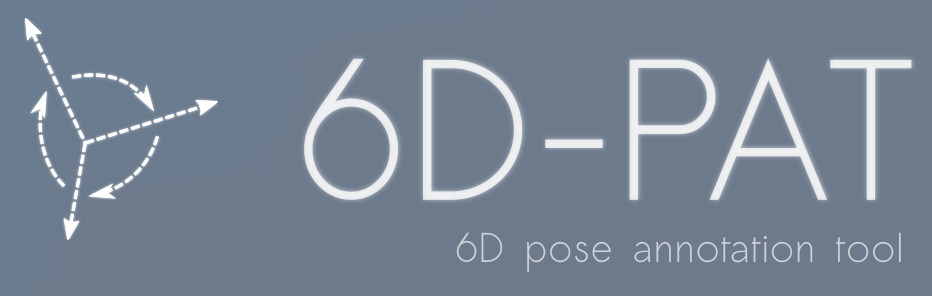
\includegraphics[width=\linewidth]{6dpat}
    \caption{The logo of the pose annotation tool 6D-PAT. Own image.}
    	\label{fig:6dpat_logo}
\end{figure} 

The following chapter analyzes manual 6D pose annotation process and its prerequisites. To this end, the necessary terminology is defined and explained and the workflow to annotate poses using the developed annotation tool is described. The assessment of the requirements of the annotation procedure and the creation of the tool are conducted based on the medical image dataset, which is described further below.

\section{Terminology} \label{section:terminology}

\textbf{Image.} An image $I$ is a 2D matrix of pixels. The pixel $u$ at position $(i, j)$ is referenced by the tuple $(x, y)$, where $x = j$ and $y = i$. The inverted notation is chosen over the common row-major matrix indexing to account for the universal  \\

\noindent\textbf{Object Model.} An \textit{object model}, or \textit{3D model}, $O$ is composed of a set of points $M \subseteq \mathbb{R}^3$ and a set of triangles $T = \{(m_1, m_2, m_3) \in M^3\}$. The real-world entity that the object model resembles is not restricted. In case of the T-Less dataset \cite{tless} the objects are mainly hardware like screws and power sockets. \\

\noindent\textbf{6D Pose.} A \textit{6D pose} $P$ is the tuple $(R, t)$, where $R$ is the 3x3 rotation matrix and $t$ the translation vector used to transform the respective object model into camera coordinates (see section \ref{objectcoordinates} for details). \\

\noindent\textbf{Correspondence.} A \textit{correspondence} is the tuple $(u, p)$, which captures the relation between a pixel $u$ of an image $I$ and an object model $O$. The pixel $u$ is the projection of the 3D point $p$ onto the image plane using the camera matrix $K$ and a pose $P$. If the pose is unknown, a set of at least three correspondences can be used to retrieve the pose computationally (see section \ref{objectcoordinates} for details). \\

\noindent\textbf{Segmentation Mask.} A segmentation mask for an image $I$ is a second image of the same size. Each position $(x, y)$ of the mask encodes the class of the pixel at $(x, y)$ in $I$. The set of classes can be defined arbitrarily. In the context of this work each class represents a type of object model. \\

\noindent\textbf{Pose Creation.} The process of creating correspondences can be performed in various ways. In this work the key operation is to create a set of correspondences and solve the implied perspective-n-point problem. \\

\noindent\textbf{Ground-Truth.} A \textit{Ground-Truth Pose} $\bar{P}$ is a 6D pose. A ground-truth pose is always created by a human instead of a machine. The ground-truth pose is the best approximation of the rotation and translation of an object model $O$ on an image $I$ of said object. It is an approximation because there can be a discrepancy between the real world object and its digital 3D representation. Distortions by the camera used to photograph the object and other influences might also not be modeled correctly or not accounted for at all. The rotation and translation error of a ground truth pose are bearable and thus are the objective for neural networks.

\section{Medical Images Dataset}

The goal of this work is to provide a system to successfully and efficiently annotate the medical images that were provided upfront. The dataset includes segmentation masks but no object models or existing pose annotations. An example image together with the corresponding segmentation mask are given in fig \ref{fig:sfb}. The dataset resembles the characteristics and quality of images from laparoscopic videos, i.e. there is no depth information present and occlusion and artifacts like motion blur can occur. The issues with this dataset are discussed in section \ref{section:6dpat_difficulties}. 

\begin{figure}[!tbp]
	\centering
	\begin{subfigure}[t]{0.47\textwidth}
	\centering
    	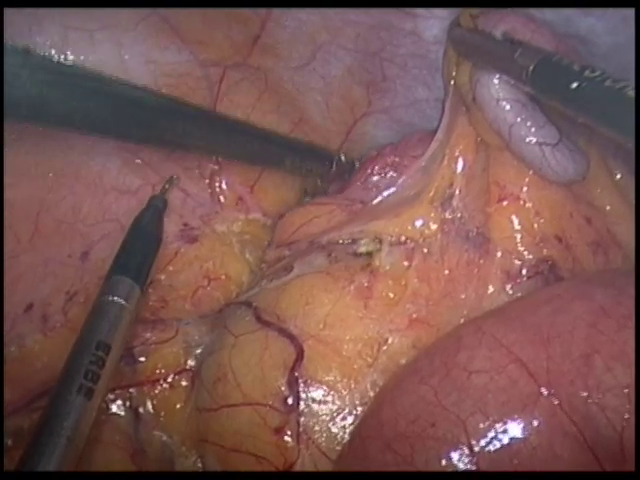
\includegraphics[width=0.8\linewidth]{sfb_original}
    	\caption{An example image from the medical dataset. Taken from TODO: cite.}
    	\label{fig:sfb_original}
	\end{subfigure}
	\hfill
	\begin{subfigure}[t]{0.47\textwidth}
	\centering
    	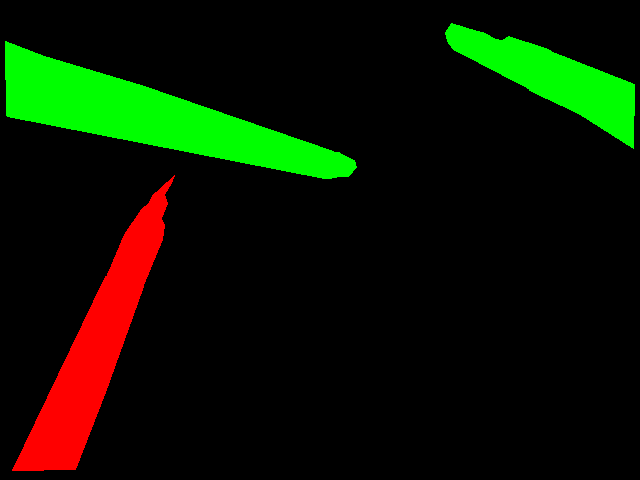
\includegraphics[width=0.8\linewidth]{sfb_segmentation}
    	\caption{The corresponding segmentation mask to the image in fig \ref{fig:sfb_original}. The colors encode the tools' classes. Taken from TODO: cite.}
    	\label{fig:sfb_segmentation}
	\end{subfigure}
	\caption{An example image and its corresponding segmentation mask from the medical dataset.}
	\label{fig:sfb}
\end{figure} 

\section{6D Pose Annotation Tool (6D-PAT)}

The creation of sufficient training data for neural networks can be a time-consuming and tedious process. Using non-specialized tools designed for other purposes, like 3D modeling programs, require the annotation personnel to get accustomed to complex user interfaces. The goal of the annotation tool is to provide a system that allows easy and efficient annotation of images, images of the medical dataset in particular. The annotated poses, the so-called \textit{Ground-Truth Poses} (see section \ref{section:terminology}), can later be used to train a neural network. The program is written in the language C++ and named \textit{6D - Pose Annotation Tool (6D-PAT)}. Its logo can be seen in fig \ref{fig:6dpat_logo}. Although the program was developed using the \textit{Linux}-based operating system \textit{Ubuntu}, it should be compilable on other systems as well.

\subsection{Requirements}

TODO.

\subsection{Frameworks \& Third-Party Libraries}

The listed frameworks are all necessary dependencies of the annotation tool. There are no dependencies other than the mentioned ones. They are not part of the repository but have to be compiled individually instead. Since all three frameworks/libraries are platform-independent the program can be compiled and run on different systems. \\

\noindent\textbf{Qt.} \textit{Qt} \cite{qt} is a powerful framework for C++ that offers a vast selection of user interface components but also general functionality that exceeds the capabilities of the standard C++ library. Qt is also chosen as the main framework because it ensures portability of C++ applications by encapsulating system calls of all kind. \\

\noindent\textbf{OpenGL.} \textit{OpenGL} \cite{opengl} is a widespread open-source 3D graphics library specification. Implementations for many operating systems exist, thus making most OpenGL using applications compilable in different environments without further modifications. \textit{Mesa 3D} \\

\noindent\textbf{OpenCV.} \textit{OpenCV} \cite{opencv} is a C++ library created for various computer vision tasks, hence the name. OpenCV provides implementations for tracking, object detection, segmentation and many more. In this work its \textit{solvePnPRansac} is used. \\

\noindent\textbf{Assimp.} \textit{Assimp} \cite{assimp} is a C++ library designed to import 3D models. The library was incorporated into the tool to ensure a broad support of 3D model formats.

\subsection{Architecture \& Code Design}

\begin{figure}[!tbp]
\end{figure} 

\begin{figure}[!tbp]
	\centering
	\begin{subfigure}[t]{0.47\textwidth}
		\centering
    	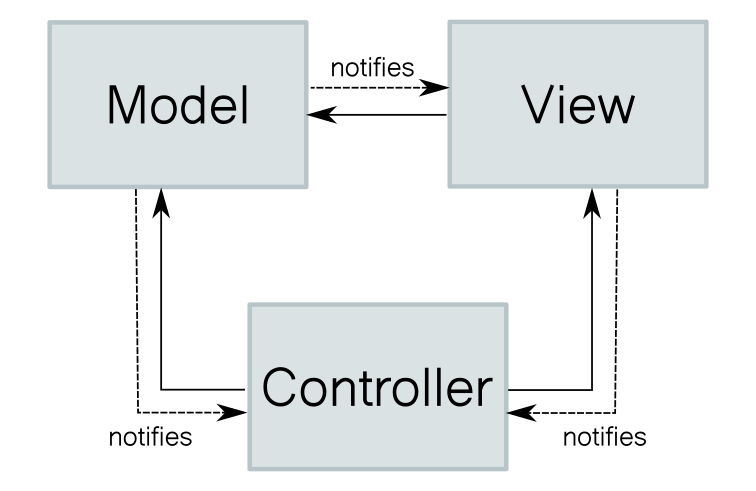
\includegraphics[width=0.8\linewidth]{mvc}
    	\caption{The Model-View-Controller architecture. The solid lines stand for a direct connection either because the target is owned or known by reference. The dashed line is an indirect connection using for example the observer pattern or the Qt Signals and Slots mechanism visible in fig. \ref{fig:qt_signals_slots}. Own image.}
    	\label{fig:mvc}
	\end{subfigure}
	\hfill
	\begin{subfigure}[t]{0.47\textwidth}
	\centering
    	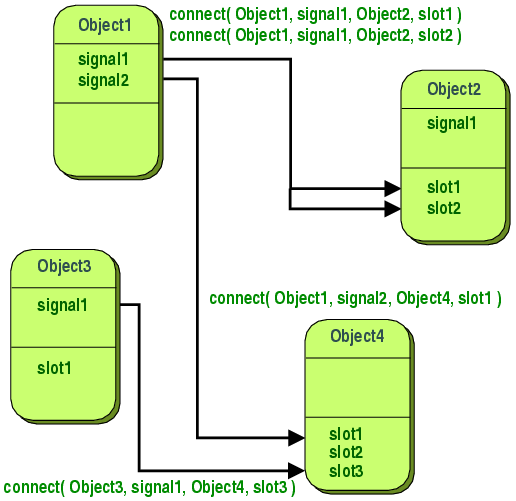
\includegraphics[width=0.8\linewidth]{qt_signals_slots}
    	\caption{The Signals and Slots mechanism of Qt. Image taken from \cite{qt_signals_and_slots}.}
    	\label{fig:qt_signals_slots}
	\end{subfigure}
\end{figure} 

6D-PAT is primarily a \textit{Graphical User Interface (GUI)} program primarily, i.e. its purpose is to display a window and enable optical interaction like clicking. Thus, the chosen underlying architecture is \textit{Model-View-Controller (MVC)}, which separates the concerns of data management (Model), displaying data (View) and high level logic (Controller). The schematic of the MVC architecture is given in fig. \ref{fig:mvc}. The indirect connections are realized via the Qt Signals and Slots mechanism, which is visualized in fig. \ref{fig:qt_signals_slots}.

% Qt Signals/Slots, Qt UI Designer

% Describe data format

\subsection{Problems \& Difficulties} \label{section:6dpat_difficulties}

During the implementation of the program multiple problems arose and complicated the development process. The most drastic ones are mentioned in this section. Issues contradicting the initial usage patterns and their impact on the final design of the program are explained, as well. \\

One of the major factors that prolong the implementation process was the usage of the only recently released \textit{Qt3D}, which is part of the Qt framework. Qt3D's purpose is to encapsulate graphics programming to increase portability of applications including 3D graphics. The incomplete documentation and unintuitive concepts make it difficult to use without consultation. After more and more complications emerged in the almost completed product the Qt3D framework was deemed unusable and omitted in favor of a native OpenGL implementation. \\

Initially, a desired feature of the program was to present a next unannotated image when the user annotated all poses of an image. This is not feasible for multiple reasons. \\

% Explain why the program does not directly present the next frame
% -> the user who was ordered to annotate wants to advance quickly
% -> profits more from the nextwork
% Why does the program not initialize the next position -> stupid

% Laggy 3D

Annotating the T-Less dataset works very well. The T-Less dataset provides high-resolution images and 3D models of the photographed objects. While trying to annotate the medical images dataset it became clear, that proper 3D models are crucial for successful annotation. To temporarily annotate the medical images, 3D surgical tools were downloaded from the internet as a replacement for the missing object models. But having a different shape and also missing the distinctive features of the real objects makes in very difficult to estimate the ground-truth pose. It is not clear what the influence of contradicting annotated poses is during training of a network. The author of this work strongly recommends to obtain the correct 3D models before annotating the medical images.

\subsection{Manual Annotation}

The next sections describe the user interface of 6D-PAT and the required steps to annotate images with 6D poses.

\subsubsection{Preparation}

% Creation of info.json

% Setting the paths to the images, to the object models and to the ground truth files

\subsubsection{Correspondence and Pose Creation}

% Describe visual structure / workflow of the program

% Click pixels u and corresponding 3D points p until enough to
% create new pose P

% Example annotations

% Proof of concept with medical images



\begin{figure}[!tbp]
	\centering
    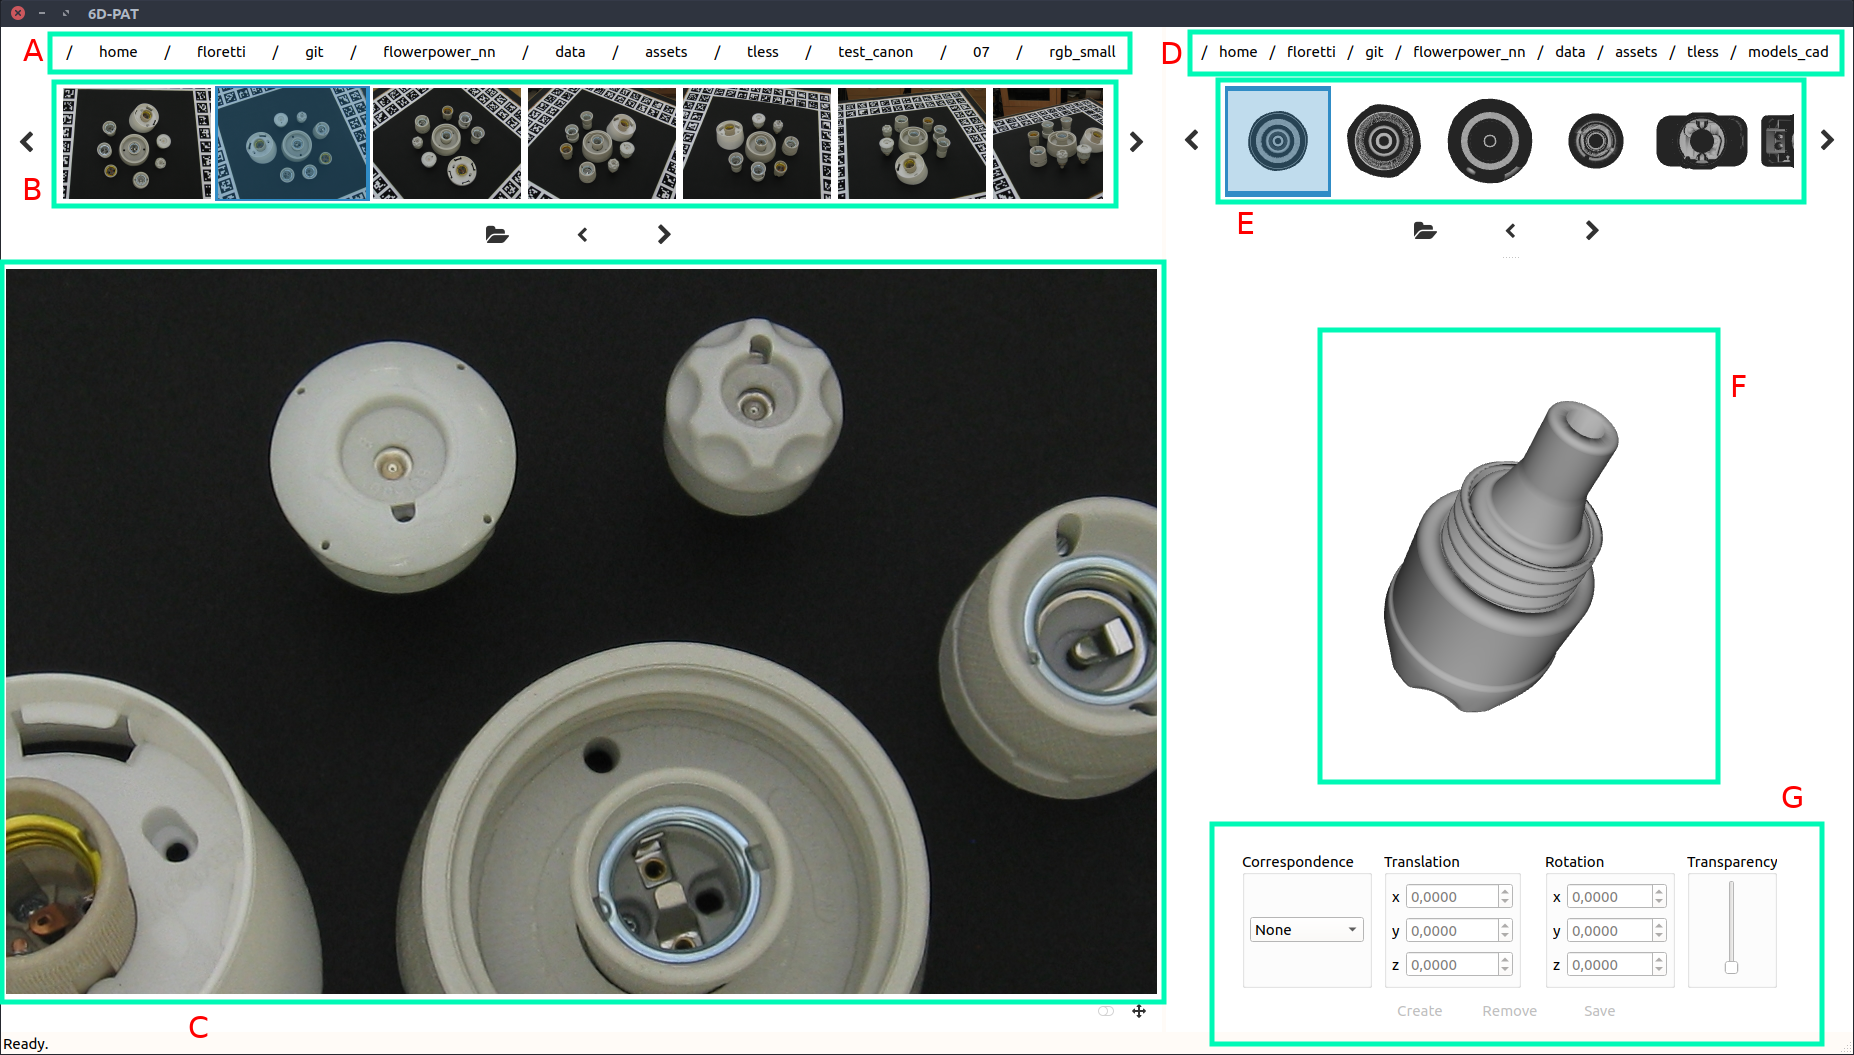
\includegraphics[width=\linewidth]{6dpat_tless_image_annotated}
    \caption{The user interface of the annotation tool 6D-PAT. The data displayed are images and object models from the T-Less dataset. Own image.}
    \label{fig:6dpat_tless_image_annotated}
\end{figure} 

\begin{figure}[!tbp]
	\centering
    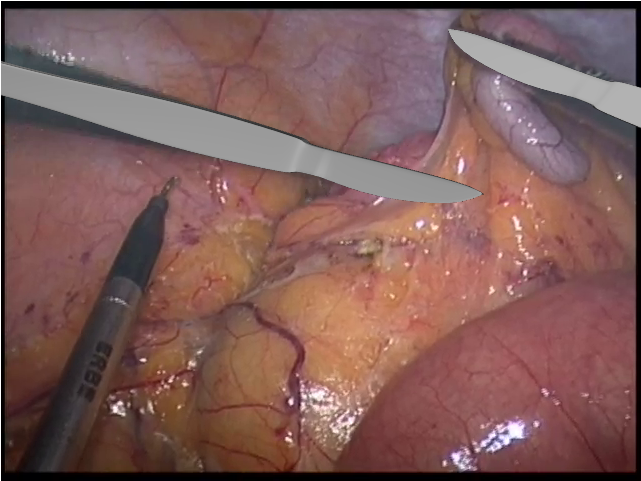
\includegraphics[width=\linewidth]{6dpat_sfb_image}
    \caption{}
    \label{fig:6dpat_sfb_image}
\end{figure} 

\begin{figure}[!tbp]
	\centering
    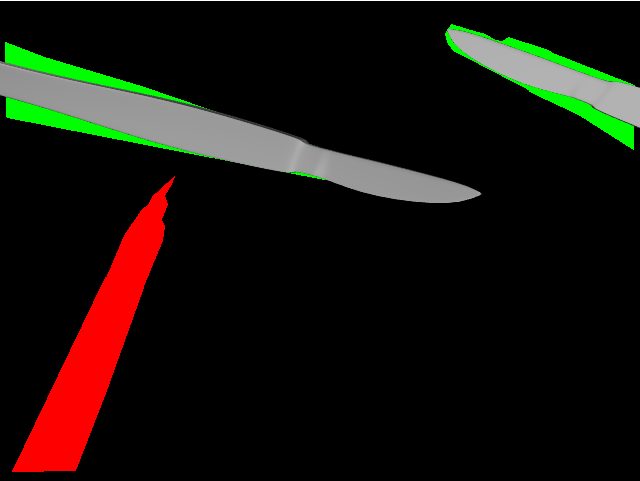
\includegraphics[width=\linewidth]{6dpat_sfb_segmentation}
    \caption{}
    \label{fig:6dpat_sfb_segmentation}
\end{figure} 

\subsection{Future Improvements}

% Inclusion of the network

% Port to python

% Movement/rotation of 3D tools by mouse